\documentclass[
	11pt, 
	DIV10,
	ngerman,
	a4paper, 
	oneside, 
	headings=normal, 
	captions=tableheading,
	final, 
	numbers=noenddot
]{scrartcl}


\usepackage[ruled]{algorithm2e}
\usepackage{graphicx}
\usepackage{hyperref}
\usepackage{amsmath}


\title{Fully Asynchronous SPH Simulation}
\subtitle{\vspace{0.5cm}Seminar: Current Topics in Fluid Animation}
\author{Yinglun Liu}


\begin{document}
\maketitle


\section{Motivation}

Over the years, the adoption of smoothed particle hydrodynamics(SPH) has developed to become the common pratice when simulating fluids in various scenes. In non-iterative approaches, the physical properties of a fluid particle is constantly influenced by its immediate neighborhood and is thus updated in each time step following a few equations of state that helps compute the components in the Navier-Stokes equation. In these equations, the computation of new attributes of the current particle requires several times the access to information from its surrounding neighbors. Intuitively, a natural practice would be to, as did many non-iterative SPH solvers, perform global updates to all particles using a single uniform time step. While iterative SPH solvers nowadays generally yield better performances, traditional non-iterative approaches do not seem to lessen in popularity due to the fact that they are easy to implement and suitable for less turbulent fluids (see Fig. \ref{fig1}).

\begin{figure}[tb]
	\centering
	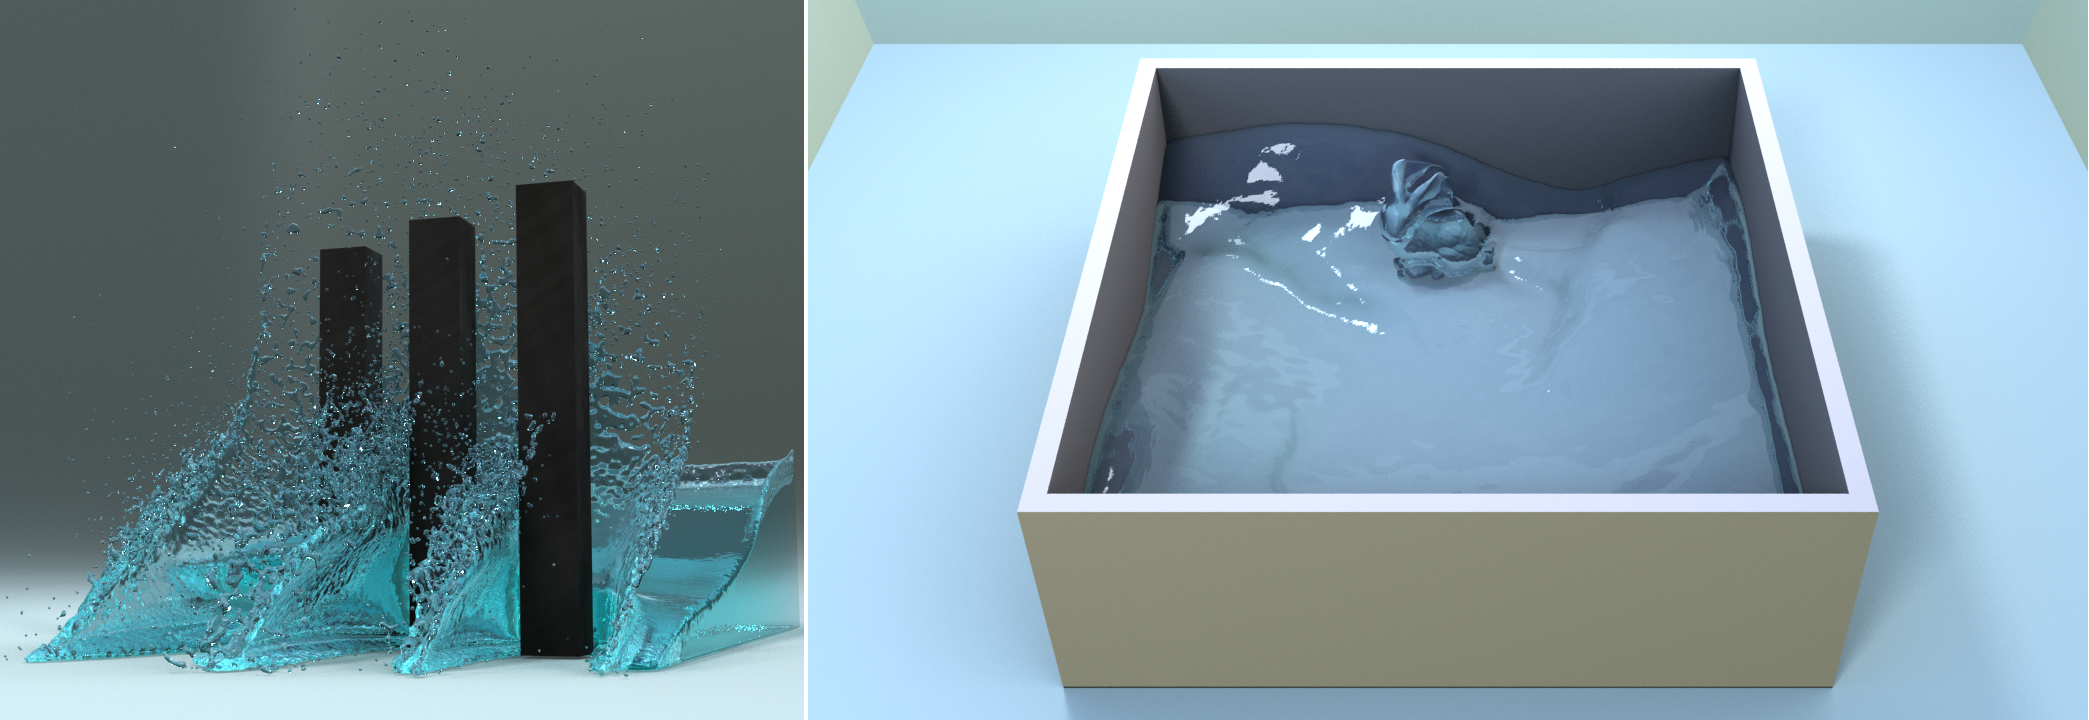
\includegraphics[scale=0.26]{images/3}
	\caption{\label{fig1} Animated scenes of dam break and radial flow demonstrate that non-iterative SPH solvers are capable of generating fluid scenes with high visual authenticity \cite{reinhardt2017fully}.
	}
\end{figure}

\par
Be that as it may, a core defect of non-iterative SPH solvers may lie in the lack of efficiency. On one hand, to enforce a constantly negligible density deviation within the fluid, large stiffness parameters are adopted to generate high pressures. Such selection of parameters demands smaller time steps and, in turn, a greater number of iterations for stable and correct particle interations. This can lead to tremendously higher overhead for the generation of visually realistic animation, where tens of millions of particles are included to allow for as fine-grained details as possible. On the other hand, the author made the observation that, while smaller time steps are essential in heavily interacting regions to guarantee stable simulation, in many less complex parts of the fluid a larger time step suffices (see Fig. \ref{fig2}). That is, the maximum possible time step for a particle varies substantially across different regions of the simulation, and it makes less sense to set one global time step for all particles, since it would inevitably be limited by the single particle with the strictest time constraint and lead to much waste of computational power. Previous works that attempted to tackle this aspect of the problem had to introduce some global synchronization barriers that improves consistency but somehow shadows the boost on performance due to waiting threads within parallel execution.

\begin{figure}[tb]
	\centering
	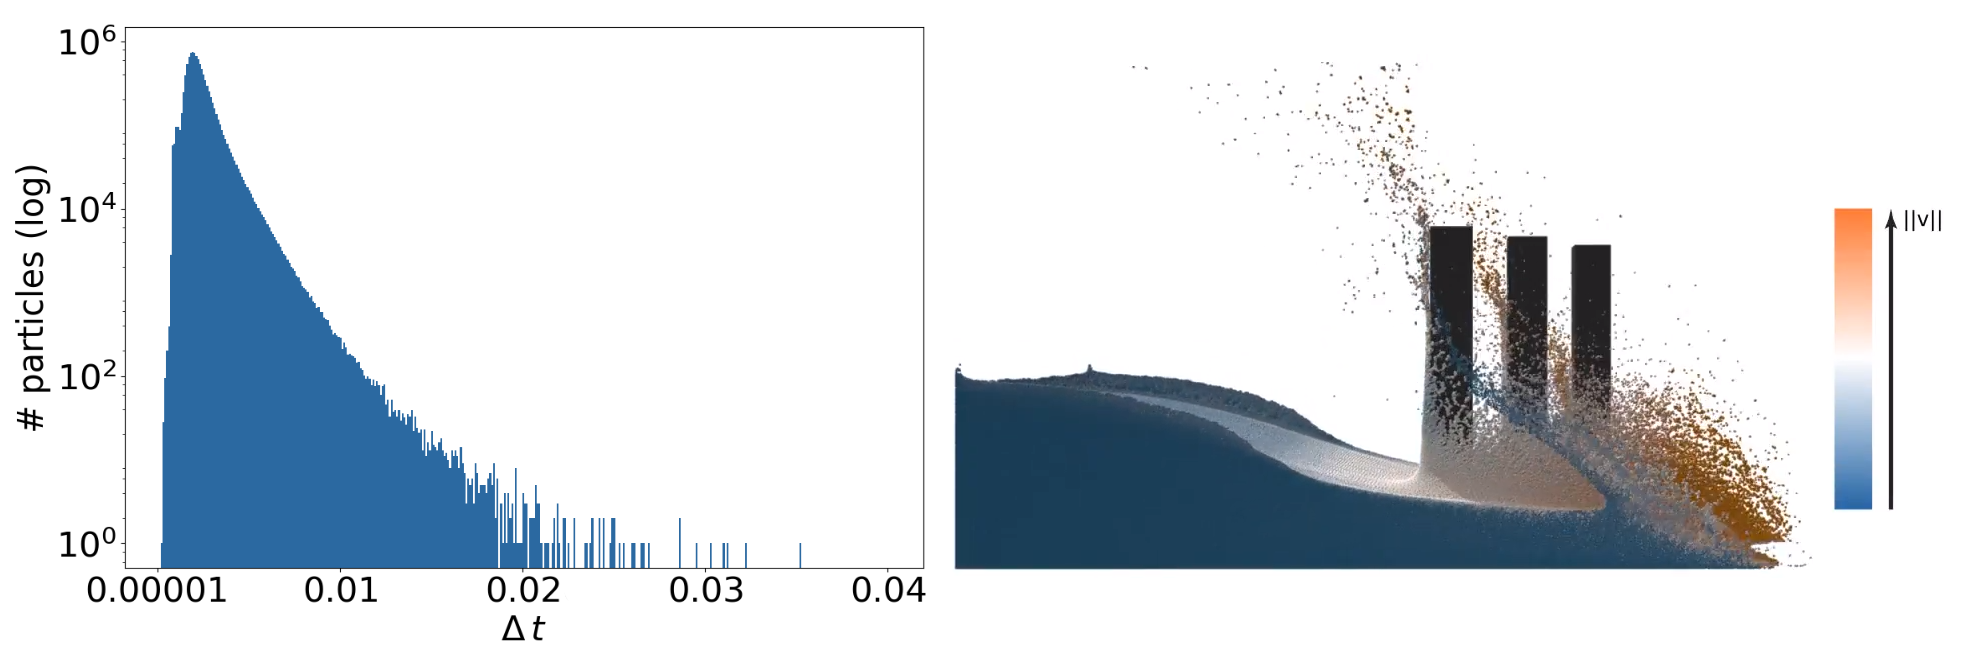
\includegraphics[scale=0.3]{images/1}
	\caption{\label{fig2} For fluid simulation based on SPH, the magnitude of velocity differs substantially across particles from different regions (right). As a result, the maximum possible time steps for each individual particle could diverge to cover up to multiple magnitudes (left) \cite{reinhardt2017fully}.}
\end{figure}

\par
To cope with this, the author proposes a novel method for the time integration of particles, in which each particle is assigned a individual time step and the whole simulation is carried out fully asynchronous. By handling each particle
individually throughout the simulation, the solver expends less computational effort on smoother regions and considerably cut down the overall time consumption. To ensure consistency, the neighborhood is reconstructed at the current time stamp each time a particle is processed. To demonstrate the strength of the proposed method, the author further proposes a multi-queue parallelization to such fully asynchronous integration procedure. Comparative experiments against related works were conducted under diverse conditions and environments to prove the efficacious enhancement on performance.

\section{Related Work}

\section{Non-iterative SPH}

Governed by the Navier-Stokes equation \ref{eq1}, non-iterative SPH performs interpolation over the neighborhood of a particle to calculate its attributes and ultimately the forces it incurs within one time step of the simulation. The fluid attribute $ A(x_{i}) $ of particle i at position $ x_{i} $ is computed as the weighted sum of  $ A(x_{j}) $ over all neighboring particles j, with the weights given by a normalizing kernel function W that is of compact support. After all forces are computed, time integration methods like symplectic Euler or leap frog is carried out to update particle position and speed.

\begin{equation}
	\label{eq1}
	\frac{\delta v}{\delta t} = -\frac{\nabla p}{\rho} + \nu v^{2} + \frac{F^{external}}{\rho}
\end{equation}

\subsection{Split Equations of State}

The author adopts here the splitting strategy as described by \cite{ihmsen2014sph}, where for each update step the advection forces $ F^{advection} $ are separately computed and then used to calculate an intermediate advection velocity $ v^{*} $. An advection density $ \rho^{*} $ is introduced to represent the expected density at the end of this time step as a result of the divergence in the velocity field if no compensating pressure force is generated. pressures $ p $ pressure forces $ F^{pressure} $ are afterwards handled conventionally. This updating scheme forces the solver to implicitly consider the impact of advection forces before generating pressure forces to counteract the deviation of density and therefore stablizes the simulation.
\par
Conventionally, a single global update step with the concept of spitting applied proceeds as in Alg. \ref{alg1}. To interpolate particle properties a neighborhood search is conducted at each time step to fetch the set of neighbors for each particle. Since such operations can be computationally expensive, spatial data
structures(e.g. a uniform grid) that supports parallel operations are usually constructed at the beginning to accelerate the process. At each global step, the grid cells are queried and updated to efficiently maintain neighborhood information. To further minimize time consumed by inevitable query operations at each time step, particles are sorted in accordance with their spatial cell. In this way, spatially adjacent particles are stored on adjacent memory slots, enhancing the cache-hit rates during the simulation. Here, the author chooses Z-order curve (see Fig. \ref{fig6}), a commonly used sorting function that effectively preserves spatial locality due to its fractal block structure, for particle indexing.

\begin{figure}[tb]
	\centering
	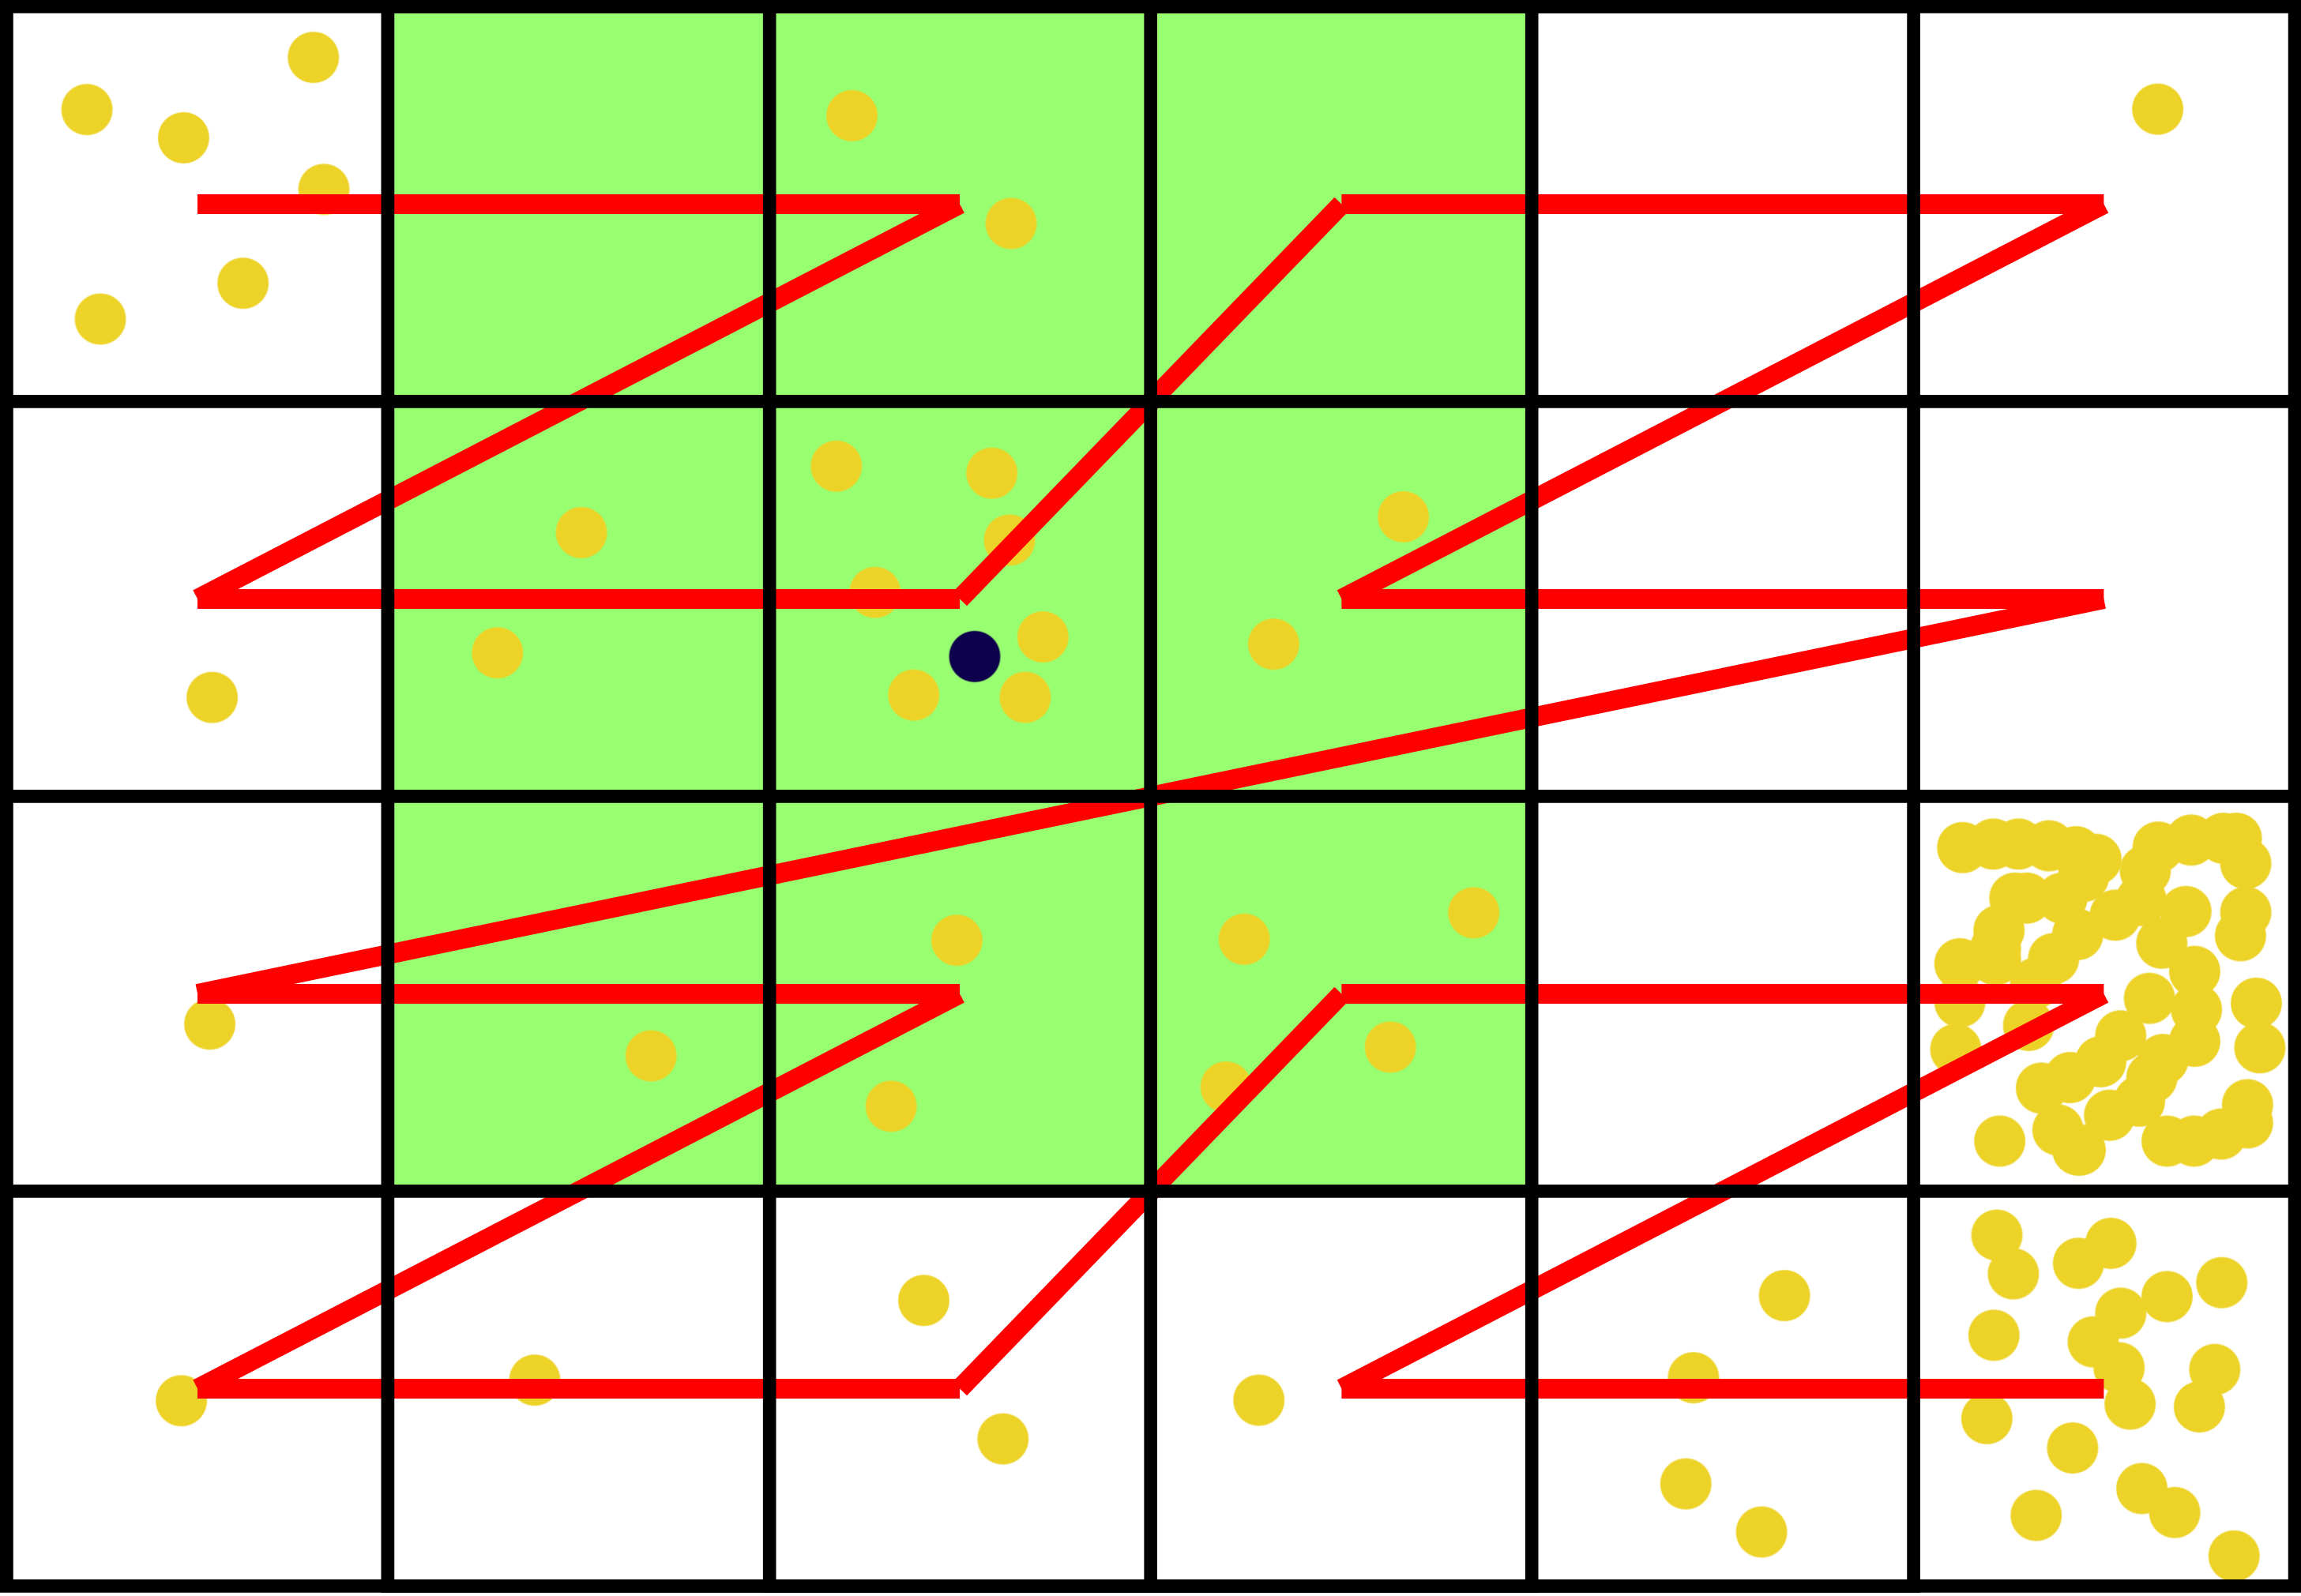
\includegraphics[scale=0.1]{images/7}
	\caption{\label{fig6} A Z-order curve in 2-dimensional space.}
\end{figure}

\large
\vskip 0.2in
\begin{algorithm}[H]
	\caption{\label{alg1} one global step with splitting \cite{reinhardt2017fully}}
	\DontPrintSemicolon
	\SetAlgoLined
	\SetKwFunction{FMain}{GlobalStep}
	\SetKwProg{Fn}{Function}{:}{}
	\Fn{\FMain{}}{
		\For{each particle i}{
			find neighbors j\;
		}
		\For{each particle i}{
			compute advection force $ F_{i}^{*} = F_{i}^{viscosity} + F_{i}^{ext} $\;
			compute advection velocity $ v_{i}^{*} $ using $ F_{i}^{*} $\;
		}
		\For{each particle i}{
			compute advection density $ \rho_{i}^{*} $\;
			compute pressure $ p_{i} $\;
		}
		\For{each particle i}{
			compute pressure force $ F_{i}^{*} $\;
			compute new particle velocity $ v_{i}(t + \delta t) $\;
			compute new particle position $ x_{i}(t + \delta t) $\;
		}
	}
\end{algorithm}
\vskip 0.2in
\normalsize

The advection force incurred by a particle consists of a viscosity component and some external components. The second-order spatial derivative of velocity reflects the diverging trend of the local velocity field and decides the viscosity component. But since second-order derivatives are tricky to compute, the approximation form proposed originally by \cite{monaghan1992smoothed} is prefered instead. Therefore the viscosity component acting on particle i is computed as

\begin{equation}
	\label{eq2}
	F_{i}^{viscosity} = 2m_{i}\nu \sum_{j}\frac{m_{j}}{\rho_{j}}v_{ij}\frac{x_{ij} \cdot \nabla W_{ij}}{x_{ij}\cdot x_{ij} + 0.01h^{2}}
\end{equation}

where $ \nu $ is a hyperparameter describing the viscocity of the liquid. Since modeling boundary interations and surface tension is not a core theme of this paper, the author directly adopts the method of \cite{akinci2012versatile} and \cite{huber2015evaluation} to handle these two aspects of the advection force.
\par
Based on the advection forces, intermediate advection velocity is computed as follows:

\begin{equation}
	\label{eq3}
	v_{i}^{*} = v_{i}(t) + \delta t\frac{F_{i}^{advection}}{m_{i}}
\end{equation}

This equation can be perceived as an intermediate velocity update using symplectic Euler without considering the impact of pressure forces. The first-order spatial derivative of velocity reflects the divergence of the velocity field and is used to compute the advection density. Again, the author chooses the robust variant presented by \cite{monaghan1992smoothed} and computes the advection density via

\begin{equation}
	\label{eq4}
	\rho_{i}^{*} = \sum_{j}m_{j}W_{ij} + \delta t_{i}\sum_{j}(v_{i}^{*} - v_{j}^{*})\cdot \nabla W_{ij}
\end{equation}

where the first term describes the static density at particle position $ x_{i} $ and the second term describes the density change during step $ \delta t_{i} $ as a consequence of diverging velocity field.
\par
Having obtained the advection densities of the particles, pressure at particle position $ x_{i} $ is computed as $ p_{i} = k(\rho_{i}^{*} - \rho_{0}) $, where $ \rho_{0} $ is the system's reference density and k is the stiffness parameter. Negative pressures are clamped to zero as in \cite{ihmsen2013implicit} to prevent the water splashes from being absorbed as a result of the induced cohesive effect. Finally, the respective pressure forces are calculated using the momentum-preserving variant:

\begin{equation}
	\label{eq5}
	F_{i}^{pressure} = -m_{i}\sum_{j}m_{j}(\frac{p_{i}}{(\rho_{i}^{*})^{2}} + \frac{p_{j}}{(\rho_{j}^{*})^{2}})\nabla W_{ij}
\end{equation}

This pressure force is then solely responsible for the explicit velocity and position update of the particle, which we discuss in the next subsection.

\subsection{Time Integration}

Despite the fact that multiple common numerical time integration schemes would fit well into the framework of non-iterative SPH solvers, the author employs a modified version of symplectic Euler:

\begin{equation}
	\label{eq6}
	v_{i}(t + \delta t) = v_{i}(t) + \delta	t\frac{F_{i}^{pressure}(t)}{m_{i}}
	x_{i}(t + \delta t) = x_{i}(t) + \delta t v_{i}(t + \delta t) + \frac{\delta t^{2}}{2}\frac{F_{i}^{pressure}(t)}{m_{i}}
\end{equation}

where in addition to a first-order tyler expansion, a second-order term is added to the position updating equation to facilitate stabler behavior when using longer time steps. For numerical stability and correct behavior of the particles, the size of each global time step has to be chosen in a way such that it fulfills the CFL condition. Intuitively, CFL condition enforces that a particle does not travel in one time step a distance that exceeds the smoothing length of the interpolating kernel. Such a constraint could guarantee that a particle does not leap over its spatial neighbors and thus fail to interact properly with them. Similarly, \cite{PE:vriphys:vriphys10:079-088} introduces a constraint on acceleration of the particle that targets the same outcome. Putting these two constraints together, the maximum time step for an individual particle is given by:

\begin{equation}
	\label{eq7}
	\delta t_{i} = min(\lambda_{v}\frac{2r_{i}}{|v_{i}|}, \lambda_{F}\sqrt{\frac{2r_{i}}{F_{i}^{pressure}/m_{i}}})
\end{equation}

where $ \lambda_{v} $ and $ \lambda_{F} $ scales the two terms respectively. In previous approaches where an globally adaptive time step is used, the system-wide time step is naturally chosen to be minimum of \ref{eq7} over all particles.


\section{Fully Asynchronous SPH}

As explained in previous sections, conventional approaches of globally fixed or adaptive time stepping squander computational resources on particles that could have been integrated with larger time steps. Former works that tries to mitigate the waste on computational power suffer from waiting threads since they introduce multiple times more synchronization barriers within the duration of the simulation. Therefore, the author proposes to assign to each individual particle a dedicated time step determined by eq. \ref{eq7} and avoid any global synchronization barrier. Only a virtual export barrier is employed from time to time to fetch particle states for rendering purposes. A comparative illustration of the proposed method is given in Fig. \ref{fig3}.

\subsection{Sequential Execution of Asynchronous Simulation}

To achieve such asynchronous SPH simulation, the solver has to constantly ensure that particle $ i $ that currently being processed has immediate access to the attributes $ A(x_{j}) $ of neighboring particles $ j $ at time stamp $ t_{i} $. Since all particles advance through time independently, this can only be achieved if the attributes of neighboring particles can be temporally interpolated. Fortunately, by employing the splitting concept, the non-iterative SPH integration already provides a feasible way to conduction such reconstruction efficiently.

\begin{figure}[tb]
	\centering
	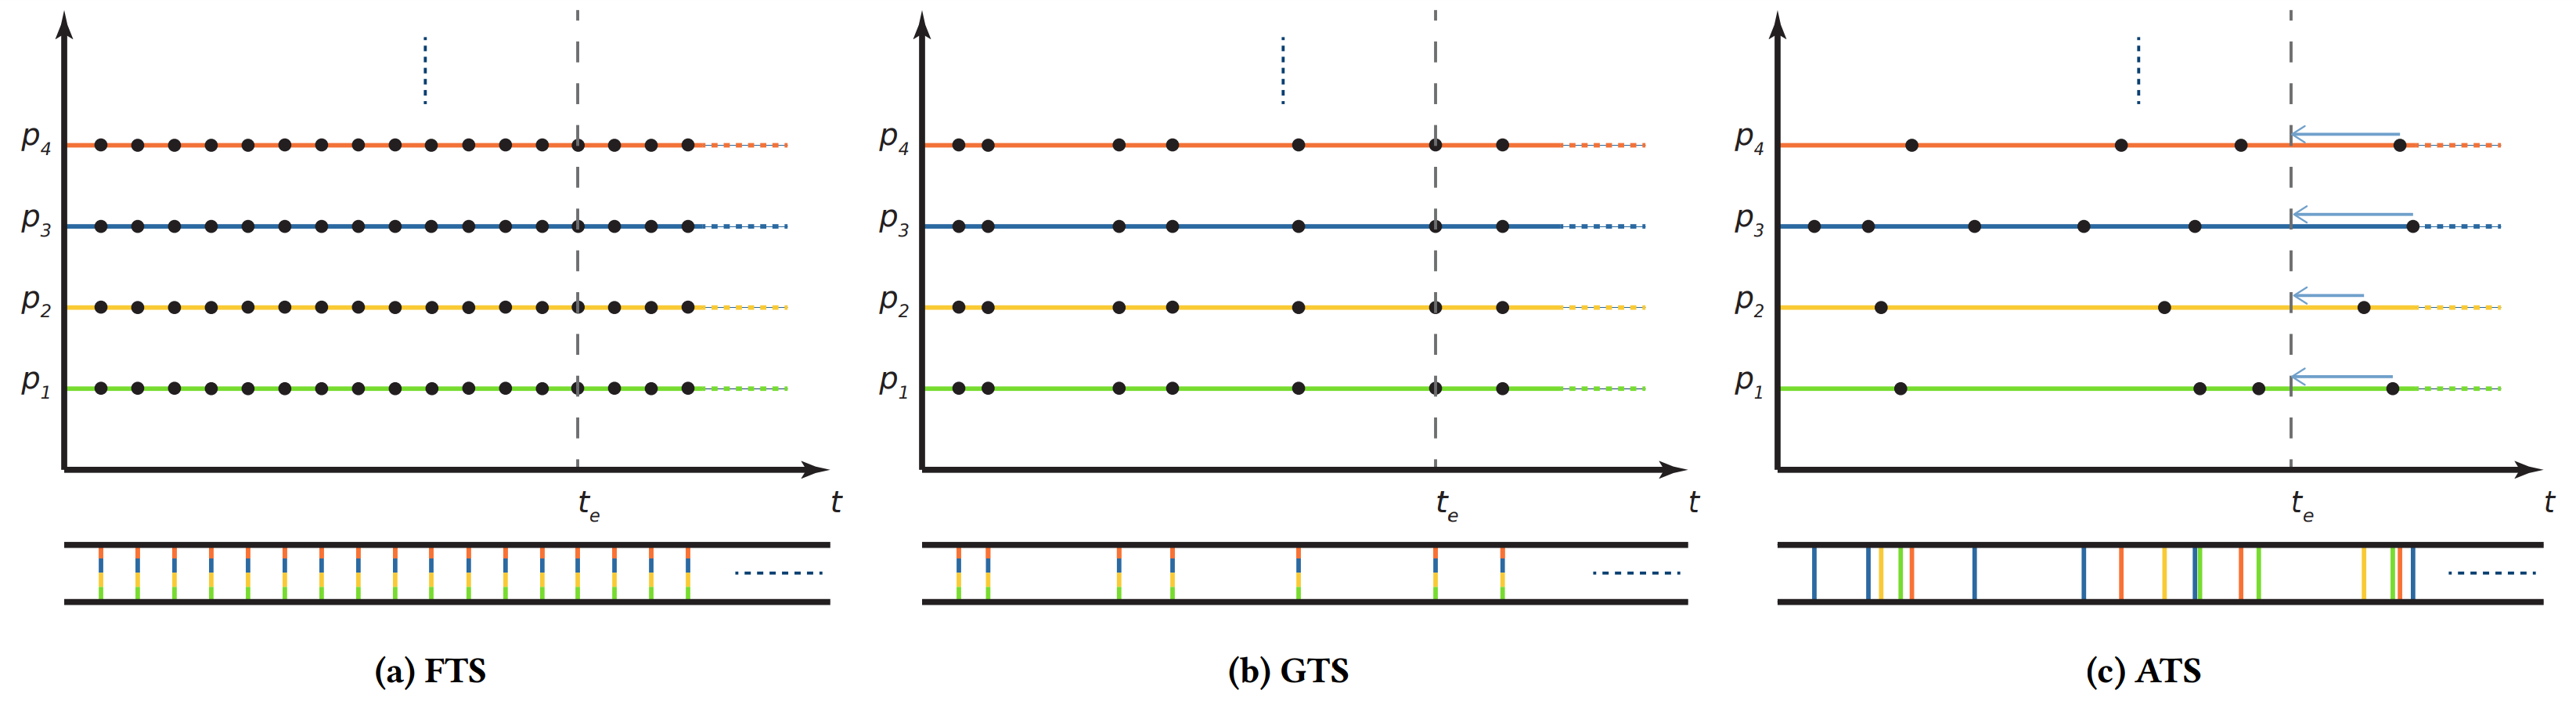
\includegraphics[scale=0.18]{images/4}
	\caption{\label{fig3} Illustration of various time stepping methods: (a) fixed time stepping (FTS), (b) globally adaptive time stepping (GTS), and (c) asynchronous time stepping (ATS). Note that with FTS and GTS all particles are updated simultaneously at each time step. With ATS each particle freely advances in time at its own pace, minimizing the overall computational expenditure. Only virtual barriers are need for exporting the outcome of the simulation. A priority queue is required to enforce a strict particle processing order for attribute consistency. \cite{reinhardt2017fully}.}
\end{figure}

\par
Similar to Alg. \ref{alg1}, one step of integration for an individual particle has the following dependencies:

\begin{itemize}
    \item the viscosity force $ F_{i}^{viscosity}(t_{i}) $ incurred by particle $i$ is dependent on the positions $ x_{j}(t_{i}) $ and velocities $ v_{j}(t_{i}) $ of neighboring particles $j$.
    \item the advection density $ \rho_{i}^{*} $ of particle $i$ is dependent on the advection velocities $ v_{j}^{*} $ of neighboring particles $j$.
    \item the pressure force $ F_{i}^{pressure}(t_{i}) $ incurred by particle $i$ is dependent on the advection densities $ \rho_{j}^{*} $ and pressures $ p_{j} $ of neighboring particles $j$.
\end{itemize}

Since velocity and position can be directly pushed forth or back in time under the symplectic Euler scheme, velocities $ v_{j} $ and positions $ x_{j} $ of neighboring particles $j$ are reconstructed at the current time stamp $ t_{i} $ to facilitate computation of viscosity force of the current particle. Since the second term in eq. \ref{eq4} approximates the temporal derivative of density, advection densities $ \rho_{j}^{*} $ of neighboring particles $j$ can be direcly pushed forth or back in time to facilitate computation of pressure force. The pressure $ p_{j} $ of neighboring particles at the current time stamp $ t_{i} $ can be computed as usual since they do not induce a high expense. Since the reconstruction of the advection velocities $ v_{j}^{*} $ of neighboring particles could be costly, we may assume that the author replaces $ v_{j}^{*}(t_{i}) $ with $ v_{j}(t_{i}) $ to cut down the total amount of operations for neighborhood reconstruction in a single particle state update. Alg. \ref{alg2} describes the outline of one individual simulation step. An illustration of the neighborhood reconstruction scheme is given in Fig. \ref{fig4}.

\begin{figure}[tb]
	\centering
	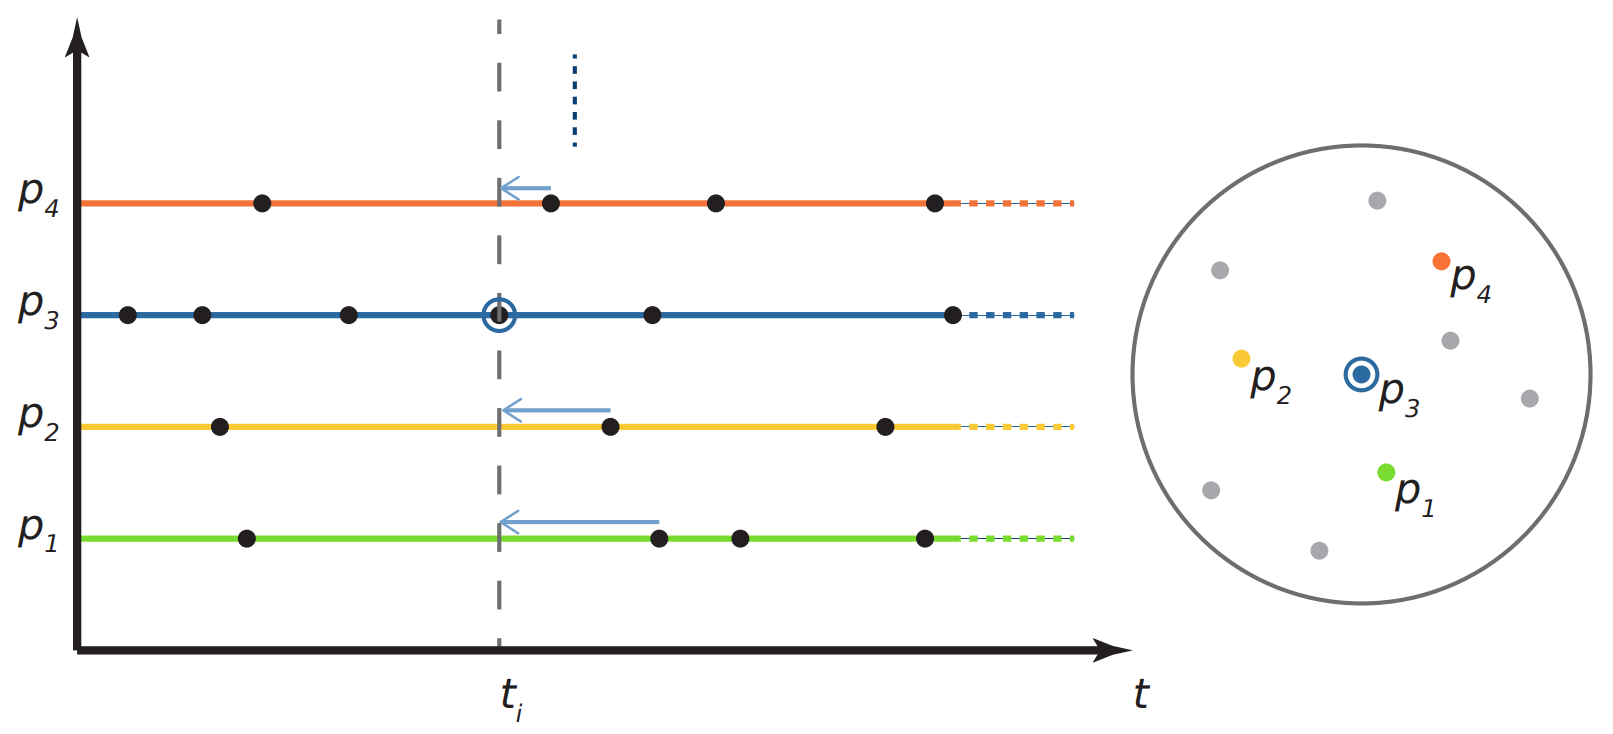
\includegraphics[scale=0.35]{images/5}
	\caption{\label{fig4} Illustration of the neighborhood reconstruction scheme: attributes of neighbors of particle $p_{3}$ are traced back in time to support the computations at the current time step. A particle is processed only when all its neighbors are already temporally ahead of itself. In this particular scenario particle $ p_{4} $ reaches the head of the priority queue after particle $p_{3}$ finishes its individual step \cite{reinhardt2017fully}.}
\end{figure}

\vskip 0.2in
\begin{algorithm}[H]
	\caption{\label{alg2} one individual step in ATS \cite{reinhardt2017fully}}
	\DontPrintSemicolon
	\SetAlgoLined
	\SetKwFunction{FMain}{IndividualStep}
	\SetKwProg{Fn}{Function}{:}{}
	\Fn{\FMain{particle $i$}}{
		\Indp
		determine maximum possible time step $ \delta t_{i} $\;
		reconstruct velocities $ v_{j}(t_{i}) $ and positions $ x_{j}(t_{i}) $ of neighbors $j$ at $t_{i}$\;
		compute viscosity force $ F_{i}^{viscosity}(t_{i}) $ incurred by particle $i$ using eq. \ref{eq2}\;
		compute external forces $ F_{i}^{ext}(t_{i}) $ incurred by particle $i$\;
		compute advection force $ F_{i}^{*}(t_{i}) $ incurred by particle $i$\;
		compute advection velocity $ v_{i}^{*}(t_{i}) $ of particle $i$ using eq. \ref{eq3}\;
		compute advection density $ \rho_{i}^{*} $ of particle $i$ using eq. \ref{eq4}\;
		compute pressure $ p_{i} = k(\rho_{i}^{*} - \rho_{0}) $ of particle $i$\;
		reconstruct advection densities $ \rho_{j}^{*} $ and pressures $ p_{j} $ of neighbors $j$ at $t_{i}$\;
		compute pressure force $ F_{i}^{pressure}(t_{i}) $ incurred by particle $i$ using eq. \ref{eq5}\;
		integrate particle $i$ over time using $ \delta t_{i} $\;
	}
\end{algorithm}
\vskip 0.2in

To guarantee stable and correct behavior of the algorithm, the author stipulates empirically that the attributes of neighboring particles should only be traced back in time. In other words, a particle is only to be processed if its entire neighborhood is more advanced in time than itself. To explicitly enforce such strict processing order, a priority queue storing only particle indices is introduced to constantly arange the particles in chronological order. Specificaly, until the next virtual export barrier is reached, the solver repeatedly dequeues the particle at the top of queue, performs one individual step for the particle and then inserts its index back into the queue such that the chronological order within the queue is sustained. After the last particle reaches the next virtual export barrier $t_{exp}$, the attributes of all particles that are demanded by the rendering process are reconstructed at $t_{exp}$ using the same procedure as stated above.

\subsection{Parallelization}

A parallel implementation of the aforementioned time stepping scheme is not straightforward given the constraint on processing order. Naively spawning multiple queues would easily lead to multiple threads stuck at each other due to the fact that a particle could have neighbors in other queues that lags behind in time and force its belonging queue to hang up until the ordinal constraint is fulfilled. To cope with this undesirably inherent character of the devised approach, the author introduces per queue a waiting list as the buffer area. When the solver of a queue runs into a particle that violates the ordinal constraint, this particle is removed and pushed into the waiting list (see Fig. \ref{fig5}). The solver then goes on to process the particle at the head of the queue until a predefined interval is reached and all particles in the waiting list are reinserted into the queue. Alg. \ref{alg3} describes the running process of a priority queue.

\begin{figure}[tb]
	\centering
	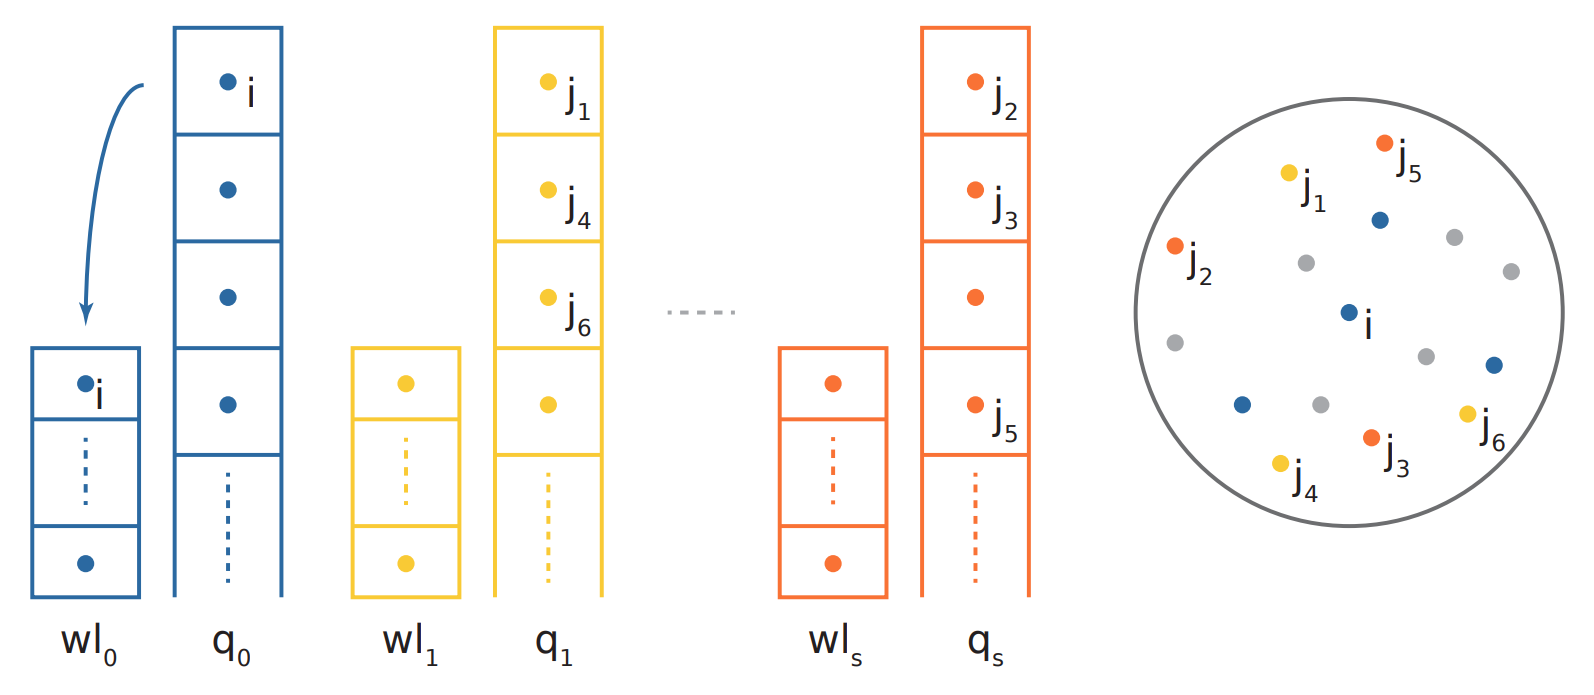
\includegraphics[scale=0.35]{images/6}
	\caption{\label{fig5} Illustration of the waiting list: the strict particle processing order could be violated when using multiple queues for parallel computation. If a particle at the head of queue $ q_{0} $ has a neighbor in another queue that is less advanced in time, the solver moves it from $ q_{0} $ and stores it on the accompanying waiting list $ wl_{0} $ \cite{reinhardt2017fully}.}
\end{figure}

\paragraph{comment}



\section{Experiments}

\section{Conclusion}

\bibliographystyle{alpha}
\bibliography{references}

\end{document}          
